\author{Andriy Zatserklyaniy, zatserkl@fnal.gov}
\documentclass[english]{article}
\usepackage{babel}
\usepackage{amsmath}
\usepackage[T1]{fontenc}
\usepackage[latin9]{inputenc}   % encoding ISO-8859-9
\usepackage{graphicx}
\usepackage{esint}              % integral symbols
\usepackage{parskip}            % for \smallskip, \medskip and \bigskip
\usepackage{cancel}             % to cancel out variables in text
\usepackage[active]{srcltx}     % enables reverse search by Shift-LeftClick in dvi file
\usepackage{listings}		% to include C++ code

%-- function to scale pictures --%
\makeatletter
\def\ScaleIfNeeded{%
\ifdim\Gin@nat@width>\linewidth
\linewidth
\else
\Gin@nat@width
\fi
}

\begin{document}

\title{Some Handy Properties of the Gaussian}

\maketitle

\section{Area of the Gaussian}

Let's consider histogram with bin width of $1/2$ units (MeV on the figure), Fig.\ref{fig:hgaus}.

\begin{figure}[h]
\centering
% \begin{minipage}[t]{0.75 \linewidth}
\begin{minipage}[t]{1.0 \linewidth}
\includegraphics[width=\ScaleIfNeeded]{hgaus.eps}
\caption{Histogram and Gaussian fit}
\label{fig:hgaus}
\end{minipage}
\end{figure}

Calculate the number of events in the histogram. 
The number of events is proportional to the histogram area
$$
S = N \cdot s_1
$$
where $s_1$ is area which corresponds to one event. 
The area of every histogram bin is a product of the bin width $w$ and the number of events in the bin.
Therefore, the area which corresponds to one event is a product of the bin width $w$ and 1: 
$$
s_1 = w \cdot 1 = w
$$
To calculate an area of the Gaussian-shape histogram in the Fig.\ref{fig:hgaus} let's approximate it by the area of the Gaussian
$$
g(x) = Ae^{-\dfrac{(x-x_0)^2}{2\sigma^2}}
$$
Fit results are:
%
\begin{align*}
A = 198.2 \\
\sigma = 0.993
\end{align*}
%
Calculate the area under the Gaussian
%
\begin{align*}
%-- I'm using & to left align the lines (default is right aligning)
S = & \int_{-\infty}^{+\infty} A e^{-\frac{(x-x_0)^2}{2\sigma^2}} \\
= & \sqrt{2\pi} \sigma A \underbrace{\int_{-\infty}^{+\infty} \frac{1}{\sqrt{2\pi}} e^{-\frac{(x-x_0)^2}{2\sigma^2}}}_{= 1} \\
= & \sqrt{2\pi} \sigma A \\
\approx & 2.5 \cdot \sigma \cdot A
\end{align*}
%
Express this area in terms of the number of events $N$ and the area of the one event $s_1$:
\begin{align*}
S = & N \cdot s_1 \\
= & N \cdot w
\end{align*}
hence
$$
N = S / w 
$$
or
$$
N = \sqrt{2\pi} \cdot \sigma \cdot A / w
$$
Because $\sqrt{2\pi} \approx 2.5066$
$$
N \approx 2.5 \cdot \sigma \cdot A / w
$$
% For the histogram on the Fig.\ref{fig:hgaus}
The histogram on the Fig.\ref{fig:hgaus} was generated for 1000 events Gaussianly-distributed with $\sigma$ = 1. 
In our approximation
\begin{align*}
\intertext{the area under the Gaussian}
S \approx 2.5 \cdot 198.2 \cdot 0.993 = 492.0 \\
\intertext{the number of events for $w$ = 0.5~MeV}
N \approx 2.5 \cdot 198.2 \cdot 0.993 / 0.5  = 984.1 \\
\end{align*}

\section{Relation between the $\sigma$ and the FWHM}

Consider a Gaussian with a mean of 0 in in the form of (see Fig.\ref{fig:fgaus}) 
% $$
% g(x) = \dfrac{1}{\sqrt{2\pi}\sigma}e^{-\dfrac{x^2}{2\sigma^2}}
% $$
$$
g(x) = Ae^{-\dfrac{x^2}{2\sigma^2}}, \qquad A = \dfrac{1}{\sqrt{2\pi}\sigma}
$$

\begin{figure}[h]
\centering
\begin{minipage}[t]{1.0 \linewidth}
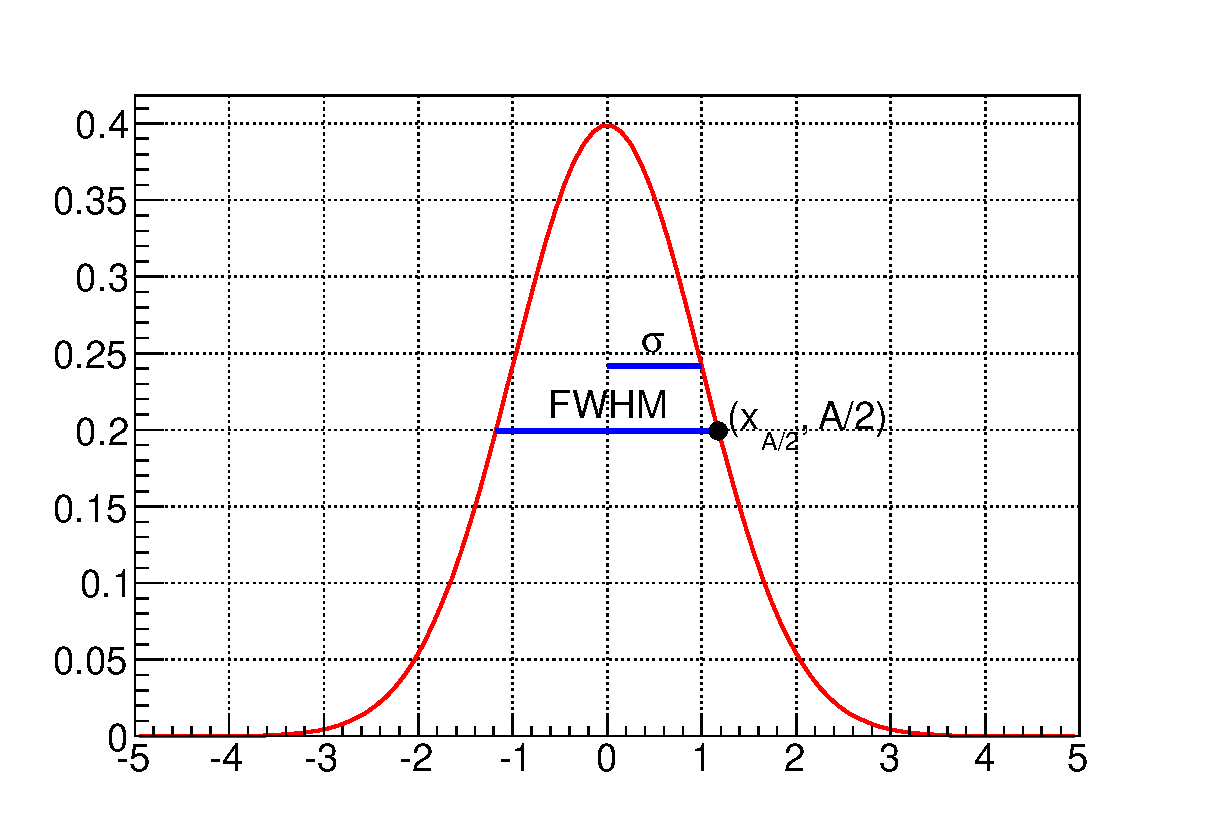
\includegraphics[width=\ScaleIfNeeded]{fgaus.eps}
\caption{Gaussian with area 1: $A = \dfrac{1}{\sqrt{2\pi}\sigma}$, mean = 0 and $\sigma=1$.}
\label{fig:fgaus}
\end{minipage}
\end{figure}

Let the Gaussian have half of the maximum value, $A/2$, at $x_{A/2}$. Then
\begin{align*}
& A/2 = Ae^{-x_{A/2}^2/2\sigma^2} \\
& log2 = \frac{x_{A/2}^2}{2\sigma^2} \\
& x_{A/2} = \sqrt{2 log 2} \cdot \sigma \\
\intertext{and}
& FWHM = 2x_{A/2} = \sqrt{8 log 2} \cdot \sigma \\
\intertext{or}
& FWHM = \sqrt{log 256} \cdot \sigma \\
\intertext{a popular approximation is}
& FWHM \approx 2.35 \cdot \sigma
\end{align*}

\section{Integral over the Gaussian}

\begin{align*}
S(x) &= \frac{1}{\sqrt{2\pi}\sigma} \int_{-\infty}^x e^{-\dfrac{t^2}{2\sigma^2}} dt \\
  &= \frac{1}{\sqrt{2\pi}\sigma} \int_{-\infty}^0 e^{-\dfrac{t^2}{2\sigma^2}} dt + 
     \frac{1}{\sqrt{2\pi}\sigma} \int_{0}^x e^{-\dfrac{t^2}{2\sigma^2}} dt \\
  &= \frac{1}{2} + \frac{1}{\sqrt{2\pi}\sigma} \int_{0}^x e^{-\frac{t^2}{2\sigma^2}} dt \\
  & \left\lvert
  \begin{aligned}
  & z = \frac{t}{\sqrt{2}\sigma} & t = \sqrt{2}\sigma z \\
  & t = x                        & dt = \sqrt{2}\sigma dz
  \end{aligned}
  \right\rvert \\
  &= \frac{1}{2} + \frac{1}{\sqrt{\cancel{2}\pi}\cancel{\sigma}} \sqrt{\cancel{2}}\cancel{\sigma} \int_{0}^x e^{-z^2} dz \\
  &= \frac{1}{2} + \frac{1}{2} \frac{2}{\sqrt{\pi}} \int_{0}^{\dfrac{x}{\sqrt{2}\sigma}} e^{-z^2} dz \\
  &= \frac{1}{2} + \frac{1}{2} erf\dfrac{x}{\sqrt{2}\sigma} \\
  &= \frac{1}{2}(1 + erf\dfrac{x}{\sqrt{2}\sigma})
\end{align*}

Finally, 
\[
S(x) = \frac{1}{2}(1 + erf\dfrac{x}{\sqrt{2}\sigma})
\]

The $S(x)$ is shown in the Fig.\ref{fig:fint_gaus}.
The error function $erf(x)$ is shown in the Fig.\ref{fig:erf}. 

Note, that 

\begin{align*}
S(-\frac{FWHM}{2}) = 0.12 \\
S(\frac{FWHM}{2}) = 0.88
\end{align*}

\begin{figure}[h]
\centering
\begin{minipage}[t]{1.0 \linewidth}
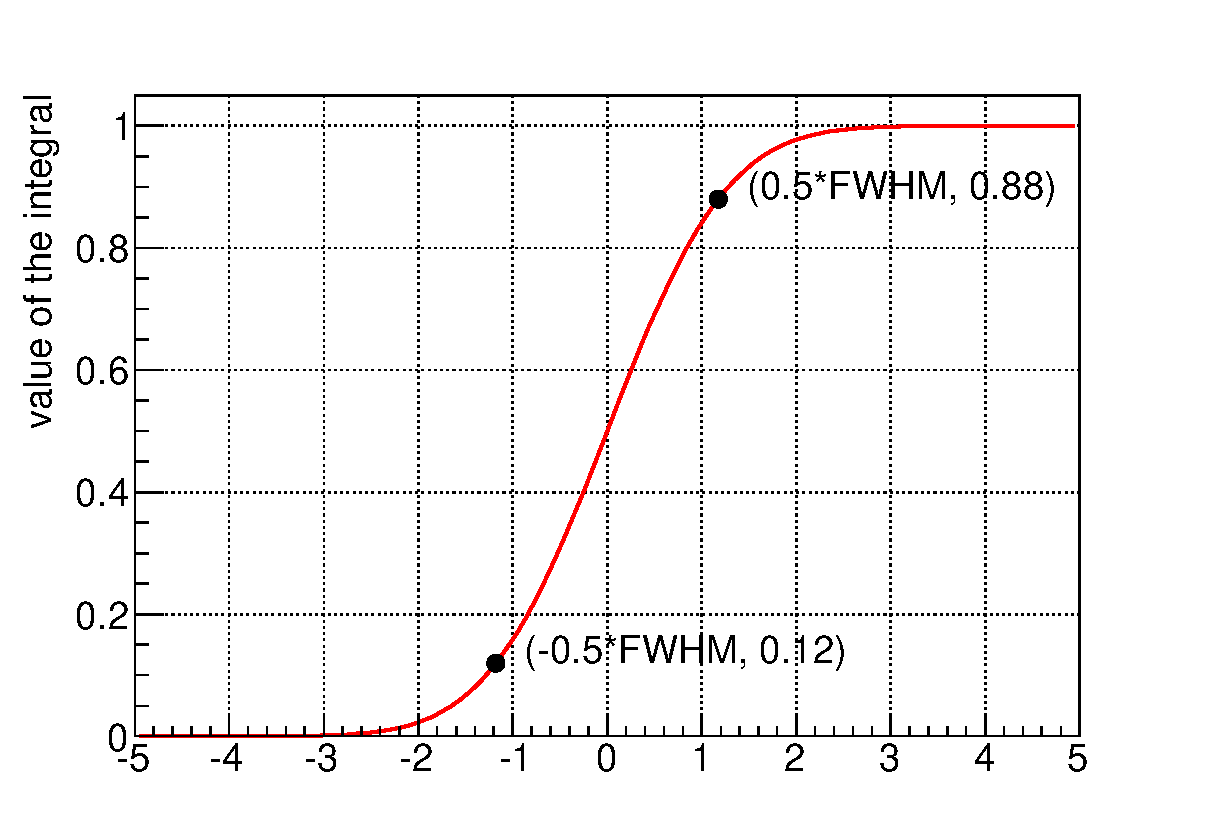
\includegraphics[width=\ScaleIfNeeded]{fint_gaus.eps}
\caption{Integral over the Gaussian $S(x) = \frac{1}{2}(1 + erf\dfrac{x}{\sqrt{2}\sigma})$}
\label{fig:fint_gaus}
\end{minipage}
\end{figure}

\begin{figure}[h]
\centering
\begin{minipage}[t]{0.75 \linewidth}
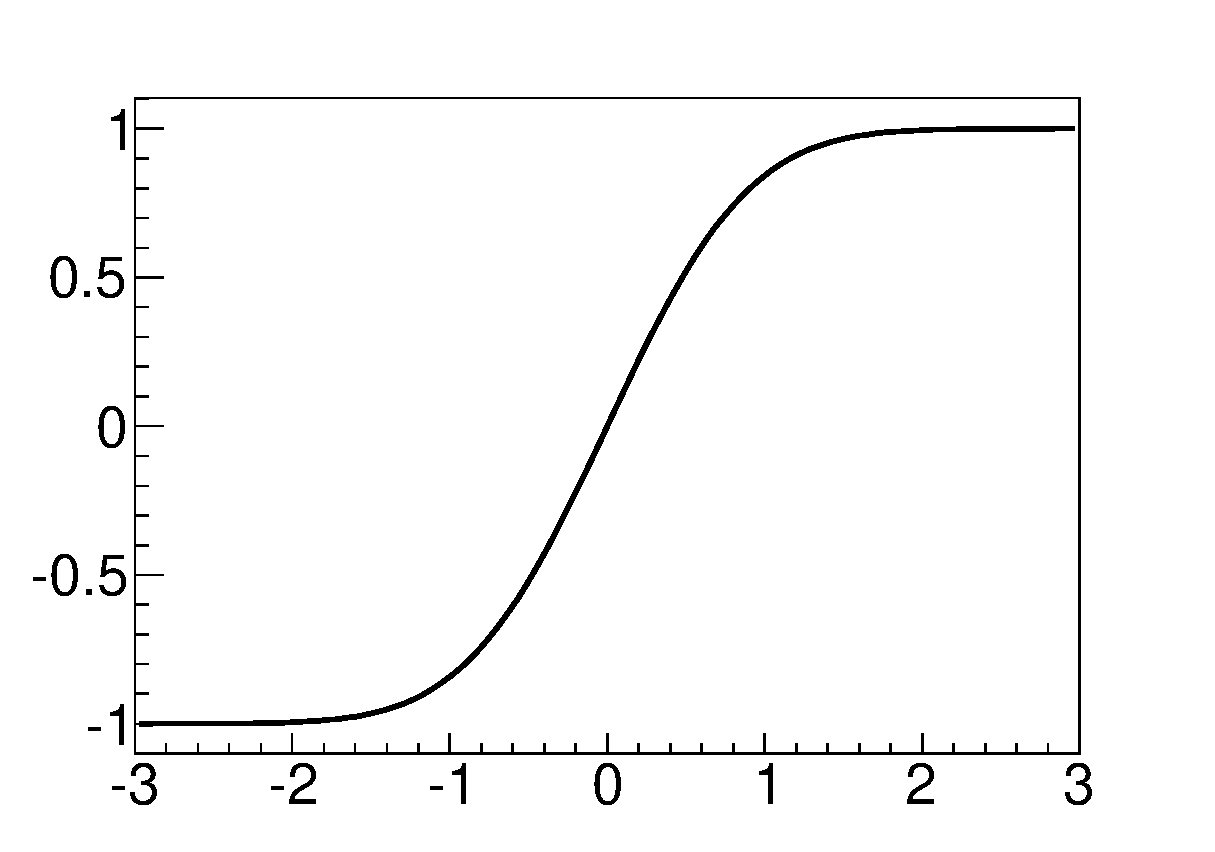
\includegraphics[width=\ScaleIfNeeded]{erf.eps}
\caption{Error function $erf(x)$}
\label{fig:erf}
\end{minipage}
\end{figure}

See Appendix~\ref{app:code_hgaus.C} for the ROOT macro code which was used to create the Figures.

% \newpage

\appendix

\section{ROOT macro hgaus.C}
\label{app:code_hgaus.C}

% see http://texblog.org/2008/04/02/include-source-code-in-latex-with-listings/

\lstset{language=C++, caption=ROOT macro hgaus.C, label=macro-hgaus.C, basicstyle=\footnotesize, frame=single, tabsize=3, breaklines=true, morecomment=[l]{//}}

% \begin{lstlisting}
% place your source code here
% \end{lstlisting}

\lstinputlisting{hgaus.C}

\end{document}
